%%=============================================================================
%% Voorbereiding op het onderzoek
%%=============================================================================

\chapter{Opzet van het onderzoek}
\label{ch:voorbereidingonderzoek}

Voor er aan de slag kan gegaan worden met het onderzoek, moet er een data warehouse opgesteld worden zowel via de Data Vault methodologie als de methodologie voor het dimensioneel modelleren. In dit hoofdstuk wordt de opbouw van het experiment uitgebreid uitgeschreven.

\section{Gebruikte technologieën in dit experiment}
De benodigdheden voor het nabootsen van dit experiment zijn:

\begin{itemize}
	\item \textbf{SAP HANA technologie:} deze databank draait op een Linux distributie (Debian) in een Azure omgeving.\footnote[1]{De SAP HANA server moet bereikbaar zijn over het internet.}
	\item \textbf{Databron:} Als databron worden csv-bestanden gebruikt die aangeleverd worden door een Windows server (versie 2016) die draait in een Azure omgeving.\footnote[2]{De Windows server moet bereikbaar zijn over het internet.}
	\item \textbf{Data Provisioning Agent:} De DP Agent wordt gebruikt om een bron te verbinden met SAP HANA.
	\item \textbf{SDI:} Een ETL-tool die aangeleverd wordt door SAP en die geïntegreerd is binnen SAP HANA.
\end{itemize}

In dit onderzoek worden voornamelijk SAP producten gebruikt. De reden hiervoor is omdat er binnen DHL Pharma Logistics ook voornamelijk gewerkt wordt met SAP producten.

\section{Overzicht van de connectie tussen SAP HANA en de host}
\begin{figure}[h]
	\centering
	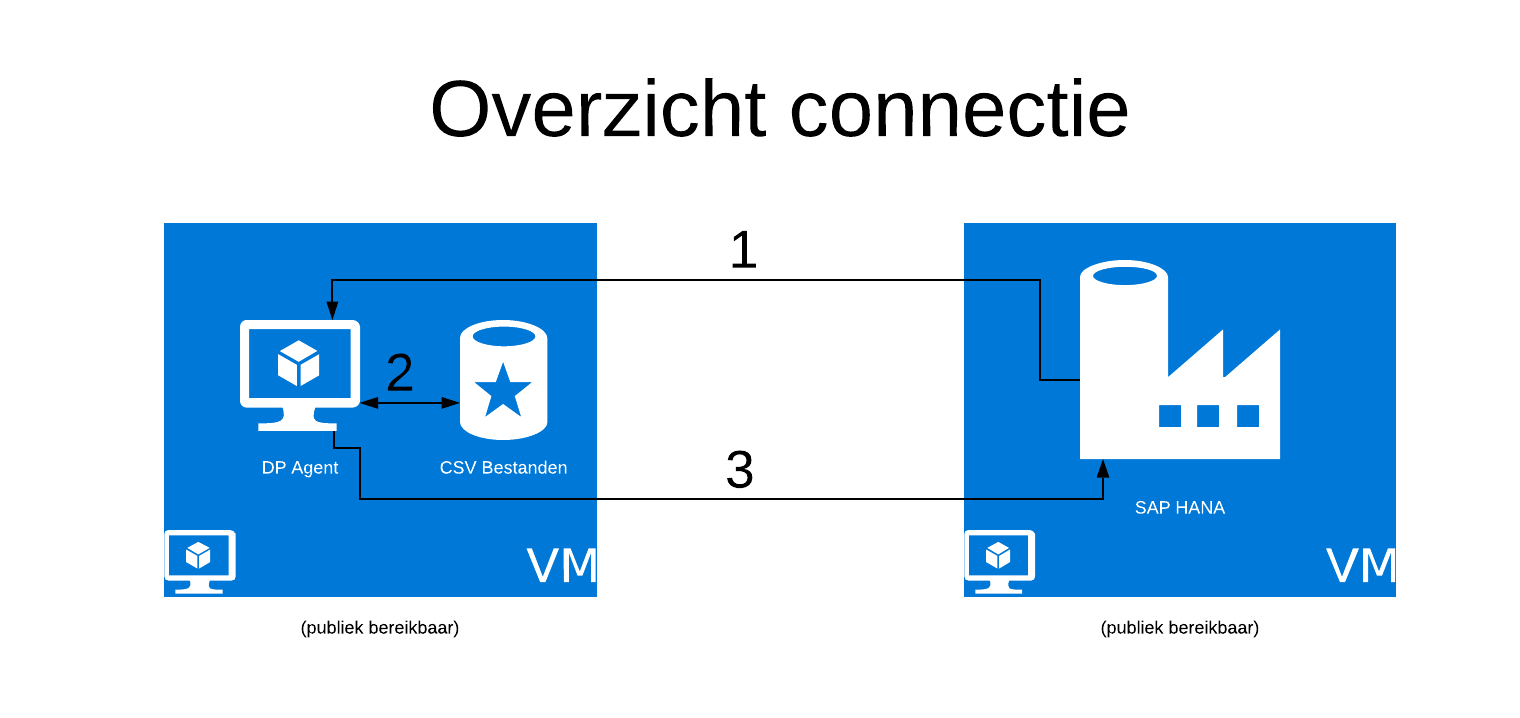
\includegraphics[scale=0.5]{../images/AzureConnectieBP.png}
	\caption{Voorstelling netwerk (gemaakt via Lucidchart.com).}
	\label{fig:azureconn}
\end{figure}

Beide virtuele machines zijn bereikbaar op het internet zodat de connectie tussen beiden mogelijk is. Op de virtuele machine waar de DP Agent op draait staat bovendien ook poort 5050 open en maakt gebruik van het TCP protocol. Dit protocol zorgt ervoor dat elk datapakket arriveert op zijn bestemming in tegenstelling tot UDP. Wanneer snelheid belangrijk (Skype, streaming, ..) is, kies je voor UDP. Dit protocol zal nooit gebruikt worden bij deze soort connectie.

Hieronder een overzicht over hoe de verbinding in zijn werk gaat:

\begin{enumerate}
	\item SAP HANA stuurt een request voor data naar de DP Agent die geïnstalleerd staat op de host.
	\item De host haalt de benodigde data op via een adapter, in dit geval haalt hij de CSV-files die nodig zijn op uit een lokale betandslocatie.
	\item De DP Agent zendt de data door naar SAP HANA.
\end{enumerate}

\section{Opzetten van een remote source}
Wanneer er een verbinding moet opgezet worden naar SAP HANA, moet een Data Provisioning Agent geïnstalleerd worden. Deze wordt geïnstalleerd op de host die een verbinding moet maken met SAP HANA. Nadat deze geïnstalleerd is, moet deze ook nog geconfigureerd worden. Volgende zaken moeten zeker in orde gebracht worden voor een connectie kan plaats vinden: 

\begin{itemize}
	\item Connection: er moet geconnecteerd en ingelogd zijn op het SAP HANA systeem.
	\item Registered: de agent moet geregistreerd zijn bij SAP HANA.
	\item Adapter: de juiste adapter (in dit onderzoek: FileAdapter) moet geregistreerd zijn bij SAP HANA. Bovendien moet de adapter ook correct geconfigureerd zijn (juiste parameters).
\end{itemize} 

\begin{figure}[h]
	\centering
	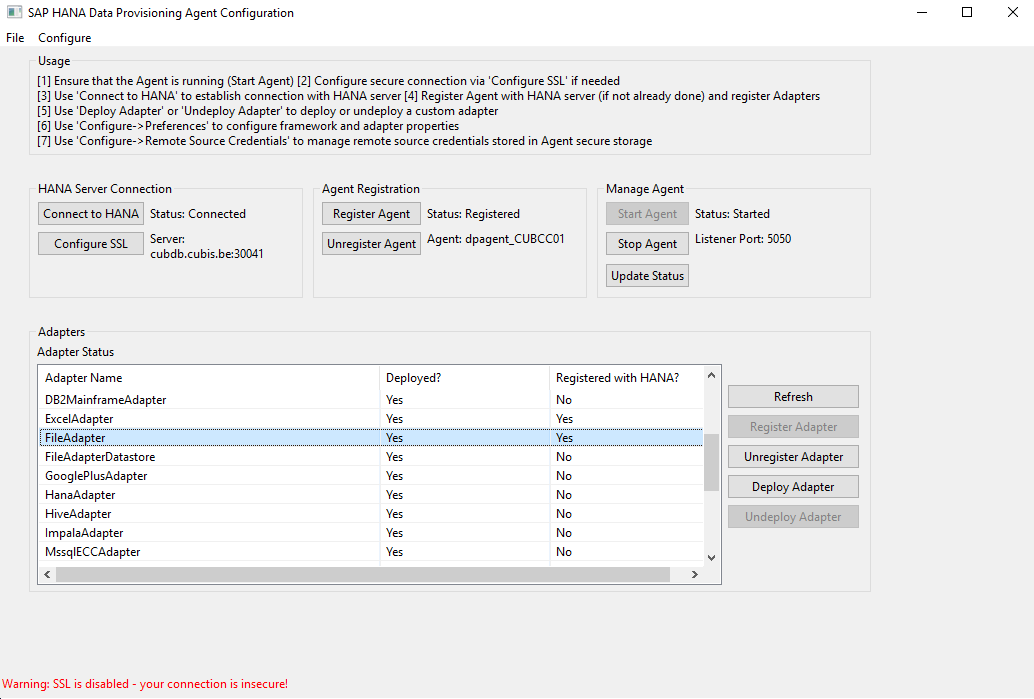
\includegraphics[scale=0.5]{../images/DPAgent.png}
	\caption{DP Agent verbonden met SAP HANA.}
	\label{fig:dpa}
\end{figure}

Wanneer alles correct geconfigureerd is, kan er nu vanuit SAP HANA een remote connectie gemaakt worden naar de host en kan de benodigde informatie opgevraagd worden.

\begin{figure}[h]
	\centering
	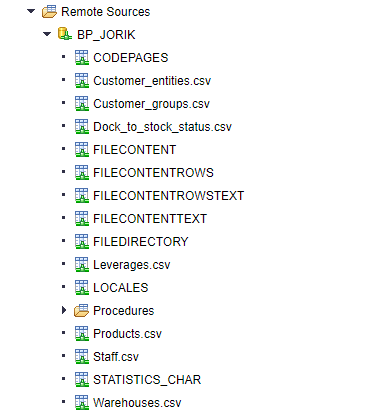
\includegraphics[scale=0.5]{../images/remoteconn.png}
	\caption{Een remote connectie opgezet naar de host vanuit SAP HANA.}
	\label{fig:remoteconn}
\end{figure}

